% option draft um zu lange Zeilen anzuzeigen
\documentclass[a4paper,11pt]{book}

\usepackage[inner=3cm,outer=3cm]{geometry}
\usepackage[english]{babel}
\usepackage[utf8]{inputenc}
% linux libertine for normal text
\usepackage{libertine}
\usepackage{libertinust1math}
% inconsolate as teletype font
\usepackage{inconsolata}
\usepackage[T1]{fontenc}
\usepackage{color}
\usepackage{graphicx}
\usepackage{wrapfig}
\usepackage{amsmath}
\usepackage{amssymb}
\usepackage{mathastext}
\usepackage{subcaption}
\usepackage{pmboxdraw}
\usepackage{lipsum}
\usepackage[export]{adjustbox}
\usepackage{csquotes}
\usepackage{tabularx}
\usepackage[sort]{natbib}
\usepackage[toc,nonumberlist]{glossaries}
\usepackage{makecell}
\usepackage[absolute,overlay]{textpos}
\usepackage{microtype}
\usepackage[linesnumbered,ruled]{algorithm2e}
\usepackage[color]{register}
\usepackage[leftbars,color]{changebar}

\setlength{\changebarwidth}{.4em}

\colorlet{tilemux}{blue!20}
\colorlet{vm}{red!20}
\colorlet{vmtilex}{orange!40}

\newcommand{\extstart}[1]{\cbcolor{#1}\cbstart}
\newcommand{\extend}{\cbend}
\newcommand{\extbox}[1]{
  \begin{tikzpicture}
    \node[draw=black, fill=#1, minimum width=.3em, minimum height=.3em] {};
  \end{tikzpicture}
}

\renewcommand{\regBitWidth}{64}
\setlength{\regWidth}{\textwidth}

% setup of siunitx
\usepackage[binary-units=true]{siunitx}
\DeclareSIUnit{\bits}{bits}
\DeclareSIUnit{\cycle}{cycle}
\DeclareSIUnit{\cycles}{cycles}
\sisetup{
  list-final-separator = {, and },
  per-mode=symbol
}

% tikz
\usepackage{tikz}
\usetikzlibrary{arrows,automata,positioning}
\usetikzlibrary{shapes.geometric}
\usetikzlibrary{shapes.multipart}
\usetikzlibrary{arrows.meta}
\usetikzlibrary{calc}
\usetikzlibrary{intersections}
\usetikzlibrary{patterns}

% tikz setup
\usepackage{environ}
\makeatletter
\newsavebox{\measure@tikzpicture}
\NewEnviron{scaletikzpicturetowidth}[1]{%
  \def\tikz@width{#1}%
  \def\tikzscale{1}\begin{lrbox}{\measure@tikzpicture}%
  \BODY
  \end{lrbox}%
  \pgfmathparse{#1/\wd\measure@tikzpicture}%
  \edef\tikzscale{\pgfmathresult}%
  \BODY
}

\makeatother
\tikzstyle{thick arrow}=[-{Latex[length=2mm]}]

% hyperlinks
\usepackage{hyperref}
\hypersetup{
  pdfauthor   = {Nils Asmussen},
  pdftitle    = {TCU Specification},
  pdfborder   = {0 0 0 [0 0]},
  colorlinks  = false
}

% listings
\usepackage{listings}
\lstset{basicstyle=\small\ttfamily,breaklines=true}
\lstdefinestyle{myc++}{
  language=C++,
  morekeywords={size_t,ssize_t}
}

% ignore page group warnings
\pdfsuppresswarningpagegroup=1

% redefine some names
\addto\extrasenglish{%
  \renewcommand{\chapterautorefname}{Chapter}%
  \renewcommand{\sectionautorefname}{Section}%
  \renewcommand{\subsectionautorefname}{Section}%
  \renewcommand{\subsubsectionautorefname}{Section}%
}

% for smart references
\newcommand{\rref}[2][]{\autoref{#2}}

% names
\newcommand{\myos}{$\text{M}^\mathbf{3}$}
\newcommand{\myfs}{$\text{M}^\mathbf{3}$FS}

% TODOs
\newcommand{\todo}[1]{\fbox{\bfseries\sffamily\scriptsize\color{red}TODO: #1}}

\title{Trusted Communication Unit -- Specification\\
\vspace{1em}Version 2.0.0}
\author{Nils Asmussen}
\date{\today}

\begin{document}

\maketitle
\tableofcontents

\chapter{System Overview}
\label{sec:systemoverview}

\newcommand{\filltile}[3]{
    \node[below=.6em of tile#1.north] {#2};
    \node[cu, above right=.6em and .6em of tile#1.south west,#3] (cu#1) {CU};
    \node[tcu,above left=.6em and .6em of tile#1.south east,#3] (tcu#1) {TCU};

    \draw[noc] ($(tile#1.south west)-(0,1.0em)$) -- ($(tile3.south east)-(0,1.0em)$);
    \draw[noc] ($(tile#1.south west)-(0,1.2em)$) -- ($(tile3.south east)-(0,1.2em)$);
    \draw[noc] ($(tile#1.south west)-(0,1.4em)$) -- ($(tile3.south east)-(0,1.4em)$);

    \draw
      let \p1=(tcu#1.south), \p2=($(tile#1.south west)-(0,1.2em)$) in
      (tcu#1.south) -- (\x1, \y2);
    \fill[radius=.2em]
      let \p1=(tcu#1.south), \p2=($(tile#1.south west)-(0,1.2em)$) in
      (\x1, \y2) circle node {};
}

\begin{figure}[h]
  \center
  \begin{tikzpicture}[
      tile/.style={draw=gray,minimum width=9.5em,minimum height=8em},
      cu/.style={draw=gray,fill=red!50,minimum width=4.5em,minimum height=4.5em},
      tcu/.style={draw=gray,fill=green!50,minimum width=3em,minimum height=3em},
      noc/.style={draw=green},
    ]

    \node[tile] (tile1) {};
    \node[tile,right=2em of tile1] (tile2) {};
    \node[tile,right=2em of tile2] (tile3) {};

    \filltile{1}{Kernel tile}{fill=green!50};
    \filltile{2}{User tile}{};
    \filltile{3}{User tile}{};

    \node[draw=black, fill=white,
          below right=.3em and .3em of cu2.north west,
          minimum width=3.9em, minimum height=3.9em] {App};

    \node[draw=black, fill=white,
          below right=.3em and .3em of cu3.north west,
          minimum width=1.8em, minimum height=1.8em] (app1) {\tiny App};
          \node[draw=black, fill=white,
          right=.3em of app1.east,
          minimum width=1.8em, minimum height=1.8em] (app2) {\tiny App};
    \node[draw=black, fill=white,
          above right=.3em and .3em of cu3.south west,
          minimum width=3.9em, minimum height=1.8em] (tilex) {Priv};
    \node[draw=black, fill=tilemux, above left=.3em and .3em of tcu3.south east] {};
    \node[draw=black, fill=vm, above left=.3em and 1.2em of tcu3.south east] {};

  \end{tikzpicture}
  \caption{System Overview.}
  \label{fig:sysoverview}
\end{figure}

\noindent The trusted communication unit~(TCU) is a building block that can be used to construct
secure systems. As shown in \rref{fig:sysoverview}, the system is based upon a tiled architecture
and each tile contains a compute unit~(CU) and a TCU. The tiles are linked through some interconnect
(e.g., a network-on-chip) and are split into \emph{kernel tiles} and \emph{user tiles}. The former
are privileged and manage the TCUs of the user tiles, whereas the latter are unprivileged.

In this system, the TCU, the interconnect, and the kernel tiles are trusted (shown green), whereas the
CUs in the user tiles are untrusted (shown red). By default, all tiles are isolated from each other, but
communication channels between tiles can be established. These communication channels can only be
establish by kernel tiles, but can be used afterwards by user tiles. Which tiles are kernel tiles is defined
by the TCU's \texttt{FEATURES} register. At boot, all tiles are kernel tiles, which can be changed by
the kernel booting on one specific tile before the other tiles start.

User tiles can have different complexities, mostly driven by the used CU. The left user tile uses a
simple core with scratchpad memory and a basic TCU without extensions. The right user tile uses a
complex core with caches and virtual memory support and a privileged software (Priv) that enables
multiple applications on the same tile and/or virtual memory. These features require TCU extensions
for virtual memory (\extbox{vm}) and/or tile sharing (\extbox{tilemux}). This specification highlights
the portions that are required by only one extension in its color and portions that are required by
either extension as \extbox{vmtilex}.

\section{Tile Internals}

\begin{figure}[h]
  \center
  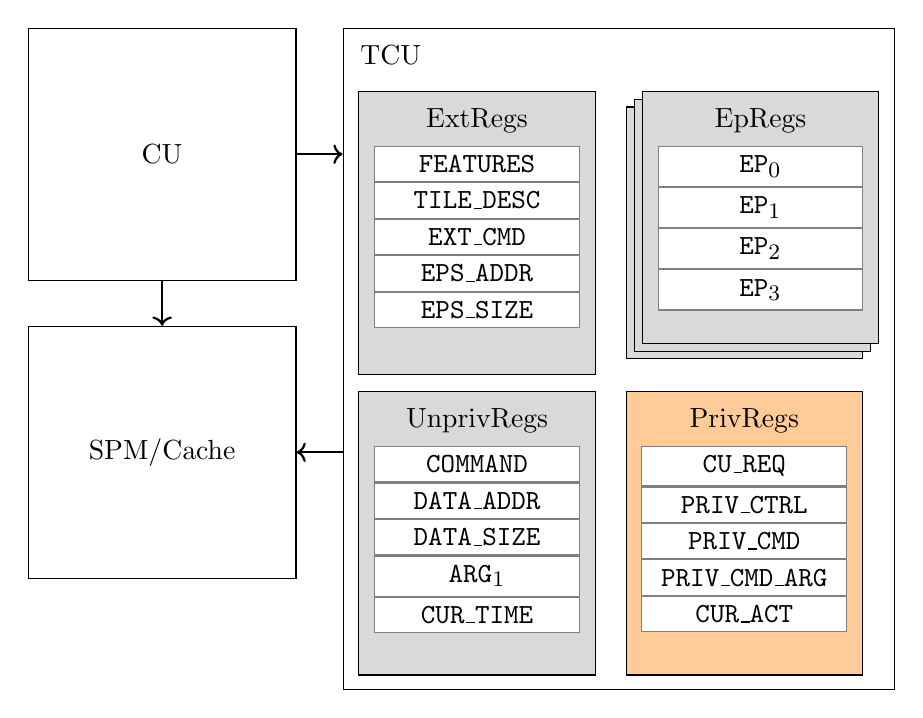
\begin{tikzpicture}[
      tcureg/.style={draw=gray,fill=white,minimum width=2.6cm},
      regtbl/.style={draw=black,fill=gray!30,minimum width=3cm}
    ]

    \node[draw=black,minimum width=7cm,minimum height=8.4cm,anchor=north west] (tcu) at(4,0) {};
    \node[draw=black,minimum width=3.4cm,minimum height=3.2cm,anchor=north west] (cu) at (0,0) {CU};
    \node[draw=black,minimum width=3.4cm,minimum height=3.2cm,anchor=south west] (mem) at (0,-7) {SPM/Cache};

    \node[below right=.1cm and .1cm of tcu.north west] {TCU};

    \node[
      regtbl,below right=.8cm and .2cm of tcu.north west,minimum height=3.6cm
    ] (tcuregs) {};
    \node[below=.1cm of tcuregs.north] {ExtRegs};
    \node[tcureg,below=.7cm of tcuregs.north] (extreg0) {\texttt{FEATURES}};
    \node[tcureg,below=0cm of extreg0]        (extreg1) {\texttt{TILE\_DESC}};
    \node[tcureg,below=0cm of extreg1]        (extreg2) {\texttt{EXT\_CMD}};
    \node[tcureg,below=0cm of extreg2]        (extreg3) {\texttt{EPS\_ADDR}};
    \node[tcureg,below=0cm of extreg3]        (extreg4) {\texttt{EPS\_SIZE}};

    \node[
      regtbl,below=.2cm of tcuregs.south,minimum height=3.6cm
    ] (cmdregs) {};
    \node[below=.1cm of cmdregs.north] {UnprivRegs};
    \node[tcureg,below=.7cm of cmdregs.north] (cmdreg0) {\texttt{COMMAND}};
    \node[tcureg,below=0cm of cmdreg0]        (cmdreg1) {\texttt{DATA\_ADDR}};
    \node[tcureg,below=0cm of cmdreg1]        (cmdreg2) {\texttt{DATA\_SIZE}};
    \node[tcureg,below=0cm of cmdreg2]        (cmdreg3) {\texttt{ARG$_1$}};
    \node[tcureg,below=0cm of cmdreg3]        (cmdreg4) {\texttt{CUR\_TIME}};

    \node[
      regtbl,below left=1cm and .4cm of tcu.north east,minimum height=3.2cm
    ] {};
    \node[
      regtbl,below left=.9cm and .3cm of tcu.north east,minimum height=3.2cm
    ] {};
    \node[
      regtbl,below left=.8cm and .2cm of tcu.north east,minimum height=3.2cm
    ] (epregs) {};
    \node[below=.1cm of epregs.north] {EpRegs};
    \node[tcureg,below=.7cm of epregs.north] (epreg0) {\texttt{EP$_0$}};
    \node[tcureg,below=0cm of epreg0]        (epreg1) {\texttt{EP$_1$}};
    \node[tcureg,below=0cm of epreg1]        (epreg2) {\texttt{EP$_2$}};
    \node[tcureg,below=0cm of epreg2]        (epreg3) {\texttt{EP$_3$}};

    \node[
      regtbl,fill=vmtilex,below right=0cm and .38cm of cmdregs.north east,minimum height=3.6cm
    ] (prvregs) {};
    \node[below=.1cm of prvregs.north] {PrivRegs};
    \node[tcureg,below=.7cm of prvregs.north] (prvreg0) {\texttt{CU\_REQ}};
    \node[tcureg,below=0cm of prvreg0]        (prvreg1) {\texttt{PRIV\_CTRL}};
    \node[tcureg,below=0cm of prvreg1]        (prvreg2) {\texttt{PRIV\_CMD}};
    \node[tcureg,below=0cm of prvreg2]        (prvreg3) {\texttt{PRIV\_CMD\_ARG}};
    \node[tcureg,below=0cm of prvreg3]        (prvreg4) {\texttt{CUR\_ACT}};

    \path
      let \p1=(cu.east), \p2=(tcu.west) in
      [draw=black,thick,->] (cu.east) -- (\x2,\y1);
    \path[draw=black,thick,->] (cu) -- (mem);
    \path
      let \p1=(mem.east), \p2=(tcu.west) in
      [draw=black,thick,<-] (mem.east) -- (\x2,\y1);
  \end{tikzpicture}
  \caption{The internal organization of a tile.}
  \label{fig:tileinternal}
\end{figure}

\rref{fig:tileinternal} shows the internals of a tile. The compute unit~(CU) is
connected to the trusted communication unit~(TCU) and can access the TCU's registers via memory
mapped input/output (MMIO). Additionally, the CU is connected to the local memory. The TCU is also
connected to the local memory (SPM or cache) to, for example, access messages. These components are
not necessarily arranged in this way. For example, the TCU might interpose itself between the CU and
local memory.

To support the security model introduced in \rref{sec:systemoverview}, the registers are split into
different groups, each group having different access permissions. All registers are generally
readable. \emph{External registers} can only be written externally, that is, from a remote tile. They
are intended for the kernel tile to manipulate the state of remote TCUs. \emph{Endpoint registers} can
be written externally and locally by the kernel tile. \emph{Unprivileged registers} can be written by
the CU. In consequence, only kernel tiles can \emph{establish} communication channels by writing
endpoint registers, but user tiles can \emph{use} these communication channels through the
unprivileged registers.

\extstart{vmtilex} The \emph{privileged registers} are intended for privileged software running on tiles
that are multiplexed among multiple activities and/or use virtual memory. The privileged software should
make sure that unprivileged software running on the same tile cannot access the privileged registers.
\extend{}

\section{Registers}

The TCU has several registers that are accessible through memory-mapped input/output~(MMIO). The
memory interface from CU to TCU is expected to be 64-bit wide. The MMIO region of the TCU is defined
as follows:

\vspace{2ex}
\noindent
\begin{tabular}{ p{3cm} | c | c | l }
  \textbf{Address} & \textbf{Register} & \textbf{Group} & \textbf{Description} \\
  \hline
  \hline
  \texttt{0xF000\_0000} & \texttt{FEATURES} & ExtRegs & Contains feature flags \\
  \texttt{0xF000\_0008} & \texttt{TILE\_DESC} & ExtRegs & Contains the tile description \\
  \texttt{0xF000\_0010} & \texttt{EXT\_CMD} & ExtRegs & Triggers external commands \\
  \texttt{0xF000\_0018} & \texttt{EPS\_ADDR} & ExtRegs & Address of endpoints region \\
  \texttt{0xF000\_0020} & \texttt{EPS\_SIZE} & ExtRegs & Size of endpoints region \\
  \hline
  \hline
  \texttt{0xF000\_0028} & \texttt{COMMAND} & UnprivRegs & Triggers unprivileged commands \\
  \texttt{0xF000\_0030} & \texttt{DATA\_ADDR} & UnprivRegs & Specifies the data address for commands \\
  \texttt{0xF000\_0038} & \texttt{DATA\_SIZE} & UnprivRegs & Specifies the data size for commands \\
  \texttt{0xF000\_0040} & \texttt{ARG$_1$} & UnprivRegs & Additional argument for commands \\
  \texttt{0xF000\_0048} & \texttt{CUR\_TIME} & UnprivRegs & Yields the current time in nanoseconds \\
  \texttt{0xF000\_0050} & \texttt{PRINT} & UnprivRegs & Triggers a debug print \\
  \hline
  \hline
  \texttt{0xF000\_0058} & \texttt{PR0} & PrintRegs & First print register \\
  \texttt{0xF000\_0060} & \texttt{PR1} & PrintRegs & Second print register \\
  \multicolumn{4}{c}{\dots} \\
  \texttt{0xF000\_0150} & \texttt{PR31} & PrintRegs & Thirty-second print register \\
  \hline
  \hline
  \texttt{0xF000\_1000} & \texttt{CU\_REQ} & PrivRegs & TCU-CU interactions \extstart{vmtilex} \\
  \texttt{0xF000\_1008} & \texttt{PRIV\_CTRL} & PrivRegs & Configures the privileged interface \\
  \texttt{0xF000\_1010} & \texttt{PRIV\_CMD} & PrivRegs & Triggers privileged commands \\
  \texttt{0xF000\_1018} & \texttt{PRIV\_CMD\_ARG} & PrivRegs & Argument for privileged commands \extend{} \\
  \texttt{0xF000\_1020} & \texttt{CUR\_ACT} & PrivRegs & Currently running activity \extstart{tilemux} \extend{} \\
  \hline
  \hline
  \texttt{0xF000\_2000} & \texttt{EP0$_0$} & EpRegs & First register of EP0 \\
  \texttt{0xF000\_2008} & \texttt{EP0$_1$} & EpRegs & Second register of EP0 \\
  \texttt{0xF000\_2010} & \texttt{EP0$_2$} & EpRegs & Third register of EP0 \\
  \texttt{0xF000\_2018} & \texttt{EP0$_3$} & EpRegs & Fourth register of EP0 \\
  \hline
  \texttt{0xF000\_2020} & \texttt{EP1$_0$} & EpRegs & First register of EP1 \\
  \texttt{0xF000\_2028} & \texttt{EP1$_1$} & EpRegs & Second register of EP1 \\
  \texttt{0xF000\_2030} & \texttt{EP1$_2$} & EpRegs & Third register of EP1 \\
  \texttt{0xF000\_2038} & \texttt{EP1$_3$} & EpRegs & Fourth register of EP1 \\
  \hline
  \multicolumn{4}{c}{\dots} \\
  \hline
  \texttt{0xF020\_1FE0} & \texttt{EP65535$_0$} & EpRegs & First register of EP65535 \\
  \texttt{0xF020\_1FE8} & \texttt{EP65535$_1$} & EpRegs & Second register of EP65535 \\
  \texttt{0xF020\_1FF0} & \texttt{EP65535$_2$} & EpRegs & Third register of EP65535 \\
  \texttt{0xF020\_1FF8} & \texttt{EP65535$_3$} & EpRegs & Fourth register of EP65535 \\
  \hline
  \hline
\end{tabular}\\[1em]

\section{Error List}

The TCU uses the following error codes to provide feedback to the software for failed commands:

\begin{itemize}
  \item \texttt{NONE} (0): no error (success),
  \item \texttt{NO\_MEP} (1): no memory endpoint,
  \item \texttt{NO\_SEP} (2): no send endpoint,
  \item \texttt{NO\_REP} (3): no receive endpoint,
  \item \texttt{FOREIGN\_EP} (4): the endpoint belongs to a different activity,
  \item \texttt{SEND\_REPLY\_EP} (5): SEND command with a reply EP or REPLY with send EP,
  \item \texttt{RECV\_GONE} (6): receiver gone (received message at non-receive EP),
  \item \texttt{RECV\_NO\_SPACE} (7): receiver buffer full,
  \item \texttt{REPLIES\_DISABLED} (8): replies are disabled,
  \item \texttt{OUT\_OF\_BOUNDS} (9): the offset and/or size is out of bounds,
  \item \texttt{NO\_CREDITS} (10): no credits to send a message,
  \item \texttt{NO\_PERM} (11): insufficient permissions,
  \item \texttt{INV\_MSG\_OFF} (12): invalid message offset,
  \item \texttt{TRANSLATION\_FAULT} (13): translation of address for data transfer failed,
  \item \texttt{ABORT} (14): a command was aborted,
  \item \texttt{UNKNOWN\_CMD} (15): unknown command,
  \item \texttt{RECV\_OUT\_OF\_BOUNDS} (16): message too large for receive buffer,
  \item \texttt{RECV\_INV\_RPL\_EPS} (17): invalid reply EPs in receive EP,
  \item \texttt{SEND\_INV\_CRD\_EP} (18): invalid credit EP in send EP,
  \item \texttt{SEND\_INV\_MSG\_SZ} (19): invalid value in msg\_sz field ($> 11$),
  \item \texttt{TIMEOUT\_MEM} (20): timeout while waiting for memory response,
  \item \texttt{TIMEOUT\_NOC} (21): timeout while waiting for NoC response,
  \item \texttt{PAGE\_BOUNDARY} (22): data to transfer contains a page boundary,
  \item \texttt{MSG\_UNALIGNED} (23): message to send is not 16-byte aligned,
  \item \texttt{TLB\_MISS} (24): entry in TLB not found,
  \item \texttt{TLB\_FULL} (25): TLB contains only fixed entries.
  \item \texttt{NO\_PMP\_EP} (26): no PMP endpoint,
  \item \texttt{NO\_IRQ} (27): no pending IRQ,
\end{itemize}

\chapter{Endpoints}

The TCU has a number of \emph{endpoints}~(EPs) to establish communication channels, which can be
configured to three different EP types: \emph{send EPs} and \emph{receive EPs} are used for message
passing, whereas \emph{memory EPs} are used for RDMA-like memory access. Each EP is represented by a
TCU register and can be configured (at runtime) to one of these EP types. Each EP consists of 256
bits, starting with 3 bits for the endpoint type (T), 16 bits for the activity that can use the EP and
237 bits (shown as dark grey below), whose meaning depends on the EP type:\\[.1em]

\begin{register}{H}{Endpoint}{}
  \regfieldb[gray!60]{}{64}{0}\regnewline%
  \regfieldb[gray!60]{}{64}{0}\regnewline%
  \regfieldb[gray!60]{}{64}{0}\regnewline%
  \regfieldb[gray!60]{}{45}{19}%
  \regfieldb[tilemux]{act}{16}{3}%
  \regfieldb{type}{3}{0}\regnewline%
  \begin{regdesc}\begin{reglist}
    \item[act] \extstart{tilemux} the id of the activity that can use this endpoint \extend{}
    \item[type] the endpoint type: INVALID (0), SEND (1), RECEIVE (2), or MEMORY (3)
  \end{reglist}\end{regdesc}
\end{register}

\section{Memory Endpoint}

\begin{register}{H}{Memory EP}{}
  \regfieldb[gray!20]{reserved}{64}{0}\regnewline%
  \regfieldb{size}{64}{0}\regnewline%
  \regfieldb{addr}{64}{0}\regnewline%
  \regfieldb[gray!20]{reserved}{27}{37}%
  \regfieldb{chip}{6}{31}%
  \regfieldb{tile}{8}{23}%
  \regfieldb{rw}{4}{19}%
  \regfieldb[tilemux]{act}{16}{3}%
  \regfieldb{type}{3}{0}\regnewline%
  \begin{regdesc}\begin{reglist}
    \item[size] the size of the region at the destination
    \item[addr] the base address of the region at the destination
    \item[chip] the destination chip ID
    \item[tile] the destination tile ID
    \item[rw] the permission bits (read = 1, write = 2)
  \end{reglist}\end{regdesc}
\end{register}

\section{Send Endpoint}

\begin{register}{H}{Send EP}{}
  \regfieldb[gray!20]{reserved}{64}{0}\regnewline%
  \regfieldb{label}{64}{0}\regnewline%
  \regfieldb[gray!20]{reserved}{34}{30}%
  \regfieldb{tgt\_chip}{6}{24}%
  \regfieldb{tgt\_tile}{8}{16}%
  \regfieldb{tgt\_ep}{16}{0}\regnewline%
  \regfieldb[gray!20]{reserved}{8}{56}%
  \regfieldb{reply}{1}{55}%
  \regfieldb{crd\_ep}{16}{39}%
  \regfieldb{msg\_sz}{6}{33}%
  \regfieldb{max\_crd}{7}{26}%
  \regfieldb{cur\_crd}{7}{19}%
  \regfieldb[tilemux]{act}{16}{3}%
  \regfieldb{type}{3}{0}\regnewline%
  \begin{regdesc}\begin{reglist}
    \item[label] the label the TCU puts into the header of each sent message
    \item[tgt\_chip] the ID of the target chip
    \item[tgt\_tile] the ID of the target tile
    \item[tgt\_ep] the ID of the receive EP at the target tile
    \item[reply] whether this is a reply EP
    \item[crd\_ep] for reply EPs: the send EP at sender-side to receive credits
    \item[max\_crd] the initially received (=max) credits (in messages)
    \item[cur\_crd] the currently owned credits (in messages)
    \item[msg\_sz] the maximum message size supported by the receiver (as power of 2)
  \end{reglist}\end{regdesc}
\end{register}

\section{Receive Endpoint}

\begin{register}{H}{Receive EP}{}
  \regfieldb{unread}{64}{0}\regnewline%
  \regfieldb{occupied}{64}{0}\regnewline%
  \regfieldb{buffer}{64}{0}\regnewline%
  \regfieldb[gray!20]{reserved}{2}{62}%
  \regfieldb{rpos}{7}{55}%
  \regfieldb{wpos}{7}{48}%
  \regfieldb{slot\_size}{6}{42}%
  \regfieldb{slots}{7}{35}%
  \regfieldb{rpl\_eps}{16}{19}%
  \regfieldb[tilemux]{act}{16}{3}%
  \regfieldb{type}{3}{0}\regnewline%
  \begin{regdesc}\begin{reglist}
    \item[unread] a bitmask with the unread (not yet fetched) messages in the buffer
    \item[occupied] a bitmask with the occupied slots in the buffer
    \item[buffer] the physical address of the receive buffer, must be 8-byte aligned
    \item[rpos] the read position (for message fetches) within the receive buffer
    \item[wpos] the write position (for message receptions) within the receive buffer
    \item[slot\_size] the size of one slot as a power of 2
    \item[slots] the number of slots in the receive buffer as a power of 2
    \item[rpl\_eps] the offset of the reply EPs
  \end{reglist}\end{regdesc}
\end{register}

\chapter{Unprivileged Interface}

The unprivileged interface of the TCU is available to unprivileged software. Most importantly, it
allows to use the TCU's endpoints via \emph{unprivileged commands}. The unprivileged registers are
used to pass input arguments for a command to the TCU, start a command, and wait until the command
is finished. The following unprivileged registers are used:

\begin{register}{H}{COMMAND}{\texttt{0xF000\_0028}}
  \regfieldb[gray!20]{reserved}{7}{57}%
  \regfieldb{arg0}{32}{25}%
  \regfieldb{error}{5}{20}%
  \regfieldb{ep}{16}{4}%
  \regfieldb{op}{4}{0}\regnewline%
  \begin{regdesc}\begin{reglist}
    \item[arg0] the first argument for the command
    \item[error] the error code (0 = no error)
    \item[ep] the endpoint to use for the command
    \item[op] the opcode of the command
  \end{reglist}\end{regdesc}
\end{register}

\noindent A write to the \texttt{COMMAND} register starts the command with opcode
\texttt{COMMAND.op} and the \texttt{DATA\_ADDR} and \texttt{DATA\_SIZE} registers specify the source
or destination data in local memory. The meaning of the two arguments (\texttt{COMMAND.arg0} and
\texttt{ARG1}) depends on the opcode.

\section{Command List}

The TCU supports the following unprivileged commands with the opcodes in parentheses. Other opcodes
lead to an \texttt{UNKNOWN\_CMD} error.

\begin{itemize}
  \item \texttt{IDLE} (0): don't do anything,
  \item \texttt{SEND} (1): send a message via a send EP to a receive EP,
  \item \texttt{REPLY} (2): reply on a message that has been received earlier via a receive EP,
  \item \texttt{READ} (3): read data from a region defined in a memory EP into local memory,
  \item \texttt{WRITE} (4): write data from local memory into a region defined in a memory EP,
  \item \texttt{FETCH} (5): fetch a new message from a receive EP,
  \item \texttt{ACK\_MSG} (6): acknowledge that the processing of a message has been completed.
\end{itemize}

\section{Pseudo Code Building Blocks}
\label{sec:unprivcmdspseudo}

The following sections use pseudo code to describe the behavior of the TCU commands, based on
several building blocks:

\begin{itemize}
  \item \texttt{read\_ep(id) -> EP}:\\
  read the TCU-internal EP register with the given id. If the id is out of bounds, an invalid EP is
  returned.
  \item \texttt{write\_ep(id, EP)}:\\
  write \texttt{EP} to the TCU-internal EP register with given id (assumed to be within bounds)
  \item \texttt{read\_local(phys, size) -> (data, Error)}:\\
  read \texttt{size} bytes from given physical address in local memory into \texttt{data} and
  return the error code (0~=~success)
  \item \texttt{write\_local(data, phys, size) -> Error}:\\
  write \texttt{data} of \texttt{size} bytes to given physical address in local memory and
  return the error code (0~=~success)
  \item \texttt{read\_remote(chip, tile, phys, size) -> (data, Error)}:\\
  read \texttt{size} bytes from the given tile on given chip at given the physical address into
  \texttt{data} and return the error code (0~=~success)
  \item \texttt{write\_remote(data, chip, tile, phys, size) -> Error}:\\
  write \texttt{size} bytes from \texttt{data} to the given physical address in the given tile on
  given chip and return the error code (0~=~success)
  \item \texttt{send\_msg(msg, chip, tile, ep)}:\\
  send \texttt{msg} to endpoint \texttt{ep} at given tile on given chip
  \item \texttt{send\_ack(error)}:\\
  send ACK to the sending TCU and report given error back
  \item \texttt{wait\_for\_ack() -> Error}:\\
  wait for the ACK the receiving TCU sends upon successfully storing the message into the receive
  buffer or an error occurred
  \item \texttt{find\_slot(mask, pos, slots, val) -> idx}:\\
  searches for a bit with value \texttt{val} in the given mask between bit 0 and bit $(1 << slots) -
  1$, starting at \texttt{pos} and rotating around. The function returns the position of the bit or
  $-1$ if none was found.
  \item \texttt{unpriv\_stop(error)}:\\
  stop the execution of the unprivileged command by setting the opcode in \texttt{COMMAND} to 0 and
  the error code to the given error.
  \item \texttt{queue\_foreign\_msg\_req(ep, act)}:\extstart{tilemux}\\
  append a new foreign-message request to the queue of CU requests (see
  \rref{code:cureqstart} for more details).\extend{}
  \item \texttt{lookup\_tlb(\colorbox{tilemux}{act, }virt, perm) -> (Phys, Error)}:\extstart{vm}\\
  lookup the given virtual address in the TLB \colorbox{tilemux}{for given activity} and return the
  physical address. On misses or missing permissions, the \texttt{TLB\_MISS} or \texttt{NO\_PERM}
  error is returned, respectively. \texttt{perm} is either \texttt{READ} or \texttt{WRITE} and denotes what permission bit needs to be present in the TLB entry. Note that the virtual address is not page aligned and the page
  offset should be added to the resulting physical address, depending on the page size set in the
  TLB entry.\extend{}
\end{itemize}

\section{Memory Access}

Memory access is performed with a memory EP based on the commands \texttt{READ} and \texttt{WRITE}.
The commands behave as follows:

\subsection{\texttt{READ}}

\begin{algorithm}[H]
    $ep \gets$ read\_ep(COMMAND.ep)\;
    \uIf{ep.type != MEMORY}{unpriv\_stop(NO\_MEP)}
    \extstart{tilemux}\uIf{ep.act != $CUR\_ACT.id$}{unpriv\_stop(FOREIGN\_EP)}\extend{}
    \uIf{ep.rw \& READ == 0}{unpriv\_stop(NO\_PERM)}
    \uIf{DATA\_SIZE == 0}{unpriv\_stop(NONE)}
    \uIf{DATA\_SIZE + $ARG_1$ > ep.size}{unpriv\_stop(OUT\_OF\_BOUNDS)}
    \extstart{vm}\uIf{(DATA\_ADDR \& 0xFFF) + DATA\_SIZE > 0x1000}{unpriv\_stop(PAGE\_BOUNDARY)}\extend{}
    \BlankLine
    $phys \gets$ DATA\_ADDR\;
    \extstart{vm}
    $(phys, err) \gets$ lookup\_tlb(\colorbox{tilemux}{CUR\_ACT.id, }DATA\_ADDR, WRITE)\;
    \uIf{err != 0}{unpriv\_stop(TRANSLATION\_FAULT)}
    \extend{}
    \BlankLine
    $(data, err) \gets read\_remote(ep.chip, ep.tile, ep.addr + ARG_1, DATA\_SIZE)$\;
    \extstart{tilemux}\uIf{err != 0}{unpriv\_stop(ABORT)}\extend{}
    $err \gets write\_local(data, phys, DATA\_SIZE)$\;
    \extstart{tilemux}\uIf{err != 0}{unpriv\_stop(ABORT)}\extend{}
    \BlankLine
    $COMMAND \gets 0$\;
    \caption{The TCU's \texttt{READ} command.}
\end{algorithm}

\subsection{\texttt{WRITE}}

\begin{algorithm}[H]
    $ep \gets$ read\_ep(COMMAND.ep)\;
    \uIf{ep.type != MEMORY}{unpriv\_stop(NO\_MEP)}
    \extstart{tilemux}\uIf{ep.act != $CUR\_ACT.id$}{unpriv\_stop(FOREIGN\_EP)}\extend{}
    \uIf{ep.rw \& WRITE == 0}{unpriv\_stop(NO\_PERM)}
    \uIf{DATA\_SIZE == 0}{unpriv\_stop(NONE)}
    \uIf{DATA\_SIZE + $ARG_1$ > ep.size}{unpriv\_stop(OUT\_OF\_BOUNDS)}
    \extstart{vm}\uIf{(DATA\_ADDR \& 0xFFF) + DATA\_SIZE > 0x1000}{unpriv\_stop(PAGE\_BOUNDARY)}\extend{}
    \BlankLine
    $phys \gets$ DATA\_ADDR\;
    \extstart{vm}
    $(phys, err) \gets$ lookup\_tlb(\colorbox{tilemux}{CUR\_ACT.id, }DATA\_ADDR, READ)\;
    \uIf{err != 0}{unpriv\_stop(TRANSLATION\_FAULT)}
    \extend{}
    \BlankLine
    $(data, err) \gets read\_local(phys, DATA\_SIZE)$\;
    \extstart{tilemux}\uIf{err != 0}{unpriv\_stop(ABORT)}\extend{}
    $err \gets write\_remote(data, ep.chip, ep.tile, ep.addr + ARG_1, DATA\_SIZE)$\;
    \extstart{tilemux}\uIf{err != 0}{unpriv\_stop(ABORT)}\extend{}
    \BlankLine
    $COMMAND \gets 0$\;
    \caption{The TCU's \texttt{WRITE} command.}
\end{algorithm}

\section{Message Passing}

Message passing is performed between a send EP and a receive EP. Each send EP is connected to
exactly one receive EP, whereas each receive EP can receive from multiple send EPs. The send EP
supports the command \texttt{SEND}, whereas the receive EP supports \texttt{REPLY}, \texttt{FETCH},
and \texttt{ACK\_MSG}.

For flow control and to prevent denial-of-service attacks on recipients, the TCU uses a credit
system. The idea is to let the recipient hand out credits to its senders, decrease the credits on
sent messages and increase them again on received replies.

Each message consists of a header and a payload. The header is built by the TCU and the payload is
given by the application. The TCU stores both header and payload into the receive buffer in memory.
The header is defined as:

\begin{register}{H}{Message Header}{}
  \regfieldb[gray!20]{reserved}{64}{0}\regnewline%
  \regfieldb{label}{64}{0}\regnewline%
  \regfieldb{rlabel}{64}{0}\regnewline%
  \regfieldb{rep}{16}{48}%
  \regfieldb{sep}{16}{32}%
  \regfieldb{length}{13}{19}%
  \regfieldb{schip}{6}{13}%
  \regfieldb{stile}{8}{5}%
  \regfieldb{rsize}{4}{1}%
  \regfieldb{flags}{1}{0}\regnewline%
  \begin{regdesc}\begin{reglist}
    \item[label] the label of the sender
    \item[rlabel] the label the receiver should use for the reply
    \item[rep] the receive endpoint ID for the reply at the sender side
    \item[sep] the sender endpoint ID
    \item[length] the payload size in bytes
    \item[schip] the sender chip ID
    \item[stile] the sender tile ID
    \item[rsize] the size of the reply message as a power of 2
    \item[flags] contains the following flags:
    \begin{itemize}
      \item \texttt{REPLY} (1): the message is a reply
    \end{itemize}
  \end{reglist}\end{regdesc}
\end{register}

\noindent The commands and the message reception behave as follows:

\subsection{\texttt{SEND}}

Note that \texttt{DATA\_SIZE == 0} is allowed and sends only the message header to the receiver
without payload. Note also the placement of \texttt{read\_local}: this transfer can fail due to
command abortions, but we haven't changed any state before. After this transfer, we reduce the
credits and send the message. The latter can again fail, but only if the receive EP is invalid or
full. If credits are not used and the receive EP is full, the state has not changed. Otherwise, the
failure indicates a broken communication channel and we consider it acceptable to leave the send EP
in a broken state, too (one credit is lost and we never get it back).

\begin{algorithm}
    $ep \gets$ read\_ep(COMMAND.ep)\;
    \uIf{ep.type != SEND}{unpriv\_stop(NO\_SEP)}
    \uIf{ep.reply != 0}{unpriv\_stop(SEND\_REPLY\_EP)}
    \extstart{tilemux}\uIf{ep.act != $CUR\_ACT.id$}{unpriv\_stop(FOREIGN\_EP)}\extend{}
    \uIf{$ep.msg\_sz > 11$}{unpriv\_stop(SEND\_INV\_MSG\_SZ)}
    \uIf{DATA\_SIZE + sizeof(header) > ($1 << ep.msg\_sz$)}{unpriv\_stop(OUT\_OF\_BOUNDS)}
    \uIf{(DATA\_ADDR \& 0xF) != 0}{unpriv\_stop(MSG\_UNALIGNED)}
    \extstart{vm}\uIf{(DATA\_ADDR \& 0xFFF) + DATA\_SIZE > 0x1000}{unpriv\_stop(PAGE\_BOUNDARY)}\extend{}
    \BlankLine
    $phys \gets$ DATA\_ADDR\;
    \extstart{vm}
    $(phys, err) \gets$ lookup\_tlb(\colorbox{tilemux}{CUR\_ACT.id, }DATA\_ADDR, READ)\;
    \uIf{err != 0}{unpriv\_stop(TRANSLATION\_FAULT)}
    \extend{}
    \BlankLine
    \uIf{COMMAND.arg\_0 != 0xFFFF}{
      $rep \gets read\_ep(COMMAND.arg_0$)\;
      \uIf{rep.type != RECEIVE}{unpriv\_stop(NO\_REP)}
      $repid \gets COMMAND.arg_0$\;
      $rsize \gets rep.slot\_size$\;
    }
    \uElse{
      $repid \gets 0xFFFF$\;
      $rsize \gets log2(sizeof(header))$\;
    }
    \BlankLine
    $(payload, err) \gets read\_local(phys, DATA\_SIZE)$\;
    \extstart{tilemux}\uIf{err != 0}{unpriv\_stop(ABORT)}\extend{}
    \BlankLine
    \uIf{ep.cur\_crd != 0x3F}{
        \uIf{ep.cur\_crd == 0}{unpriv\_stop(NO\_CREDITS)}
        $sepid \gets COMMAND.ep$\;
    }
    \uElse{
        $sepid \gets 0xFFFF$\;
    }
    \caption{The TCU's \texttt{SEND} command.}
\end{algorithm}

\begin{algorithm}
    \setcounter{AlgoLine}{37}
    $header \gets$ \{ flags $\gets$ 0\;
    $\quad\quad\quad\quad\quad label \gets ep.label$\;
    $\quad\quad\quad\quad\quad length \gets DATA\_SIZE$\;
    $\quad\quad\quad\quad\quad rsize \gets rsize$\;
    $\quad\quad\quad\quad\quad rlabel \gets ARG_1$\;
    $\quad\quad\quad\quad\quad schip \gets ownChip$\;
    $\quad\quad\quad\quad\quad stile \gets ownTile$\;
    $\quad\quad\quad\quad\quad sep \gets sepid$\;
    $\quad\quad\quad\quad\quad rep \gets repid$ \}\;
    $send\_msg(header\ |\ payload, ep.tgt\_chip, ep.tgt\_tile, ep.tgt\_ep)$\;
    $err \gets wait\_for\_ack()$\;
    \uIf{err != 0}{unpriv\_stop(err)}
    \BlankLine
    \uIf{ep.cur\_crd != 0x3F}{
        ep.cur\_crd -= 1\;
        $write\_ep(COMMAND.ep, ep)$\;
    }
    \BlankLine
    $COMMAND \gets 0$\;
    \caption{The TCU's \texttt{SEND} command (continued).}
\end{algorithm}

\newpage
\subsection{\texttt{RECEIVE}}

Note that \texttt{RECEIVE} is not a command, but just the logic at the receiver side that accepts
and stores messages. Nevertheless, its behavior is described by the following algorithm:

\begin{algorithm}[H]
    $ep \gets$ read\_ep(rep)\;
    \uIf{ep.type != RECEIVE}{send\_ack(RECV\_GONE) and drop message}
    \uIf{$sizeof(header) + header.length > (1 << ep.slot\_size)$}{send\_ack(RECV\_OUT\_OF\_BOUNDS) and drop message}
    \uIf{ep.rpl\_eps != 0xFFFF and $ep.rpl\_eps + (1 << ep.slots) > EP\_COUNT$}{send\_ack(RECV\_INV\_RPL\_EPS) and drop message}
    \BlankLine
    $idx \gets$ find\_slot(ep.occupied, ep.wpos, ep.slots, 0)\;
    \uIf{idx == -1}{send\_ack(RECV\_NO\_SPACE) and drop message}
    $ep.occupied.set\_bit(idx)$\;
    $ep.wpos \gets idx + 1$\;
    \BlankLine
    $dest \gets ep.buffer + (idx << ep.slot\_size)$\;
    $write\_local(header\ |\ payload, dest, sizeof(header) + header.length)$\;
    $ep.unread.set\_bit(idx)$\;
    $write\_ep(rep, ep)$\;
    \BlankLine
    \uIf{(header.flags \& REPLY) == 0 and ep.rpl\_eps != 0xFFFF and header.rep != 0xFFFF}{
      $sep \gets \{\ type \gets SEND$\;
      \extstart{tilemux}
      $\quad\quad\quad\ \ \  act \gets ep.act$\;
      \extend{}
      $\quad\quad\quad\ \ \  reply \gets 1$\;
      $\quad\quad\quad\ \ \  tgt\_chip \gets header.schip$\;
      $\quad\quad\quad\ \ \  tgt\_tile \gets header.stile$\;
      $\quad\quad\quad\ \ \  tgt\_ep \gets header.rep$\;
      $\quad\quad\quad\ \ \  label \gets header.rlabel$\;
      $\quad\quad\quad\ \ \  msg\_sz \gets header.rsize$\;
      $\quad\quad\quad\ \ \  max\_crd \gets 1$\;
      $\quad\quad\quad\ \ \  cur\_crd \gets 1$\;
      $\quad\quad\quad\ \ \  crd\_ep \gets header.sep$\ \}\;
      $write\_ep(ep.rpl\_eps + idx, sep)$\;
    }
    \BlankLine
    \uIf{(header.flags \& REPLY) != 0 and header.rep != 0xFFFF}{
      $sep \gets read\_ep(header.rep)$\;
      sep.cur\_crd += 1\;
      $write\_ep(header.rep, sep)$\;
    }
    $send\_ack(NONE)$\;
    \extstart{tilemux}
    \BlankLine
    \uIf{ep.act == CUR\_ACT.id}{
      CUR\_ACT.msgs += 1\;
    }
    \uElse{
      $queue\_foreign\_msg\_req(rep, ep.act)$\;
    }
    \extend{}
    \caption{If `header | payload' is received via EP `rep'.}
\end{algorithm}

\subsection{\texttt{REPLY}}

Note that \texttt{DATA\_SIZE == 0} is allowed and sends only the message header to the receiver
without payload. Like for \texttt{SEND}, note also the placement of \texttt{read\_local} and places
where state is changed. Note also that replies that fail on the reply-receiving side cannot be
repeated, because the reply EP will already be invalid. This is required to avoid a race: if the
receive-buffer slot is free'd after giving the credits back, the sender could send another message
before the slot is free. However, errors on the reply-receiving side can only be caused due to
misconfiguration anyway (receive EP invalid, not enough space in receive buffer, etc.). 

\begin{algorithm}
    $ep \gets$ read\_ep(COMMAND.ep)\;
    \uIf{ep.type != RECEIVE}{unpriv\_stop(NO\_REP)}
    \uIf{ep.rpl\_eps == 0xFFFF}{unpriv\_stop(REPLIES\_DISABLED)}
    \uIf{$ep.rpl\_eps + (1 << ep.slots) > EP\_COUNT$}{unpriv\_stop(RECV\_INV\_RPL\_EPS)}
    \extstart{tilemux}\uIf{ep.act != $CUR\_ACT.id$}{unpriv\_stop(FOREIGN\_EP)}\extend{}
    \BlankLine
    $idx \gets COMMAND.arg_0 >> ep.slot\_size$\;
    \uIf{idx >= $1 << ep.slots$}{unpriv\_stop(INV\_MSG\_OFF)}
    $sep = read\_ep(ep.rpl\_eps + idx)$\;
    \uIf{sep.type != SEND}{unpriv\_stop(NO\_SEP)}
    \uIf{sep.reply == 0}{unpriv\_stop(SEND\_REPLY\_EP)}
    \uIf{sep.crd\_ep != 0xFFFF and $sep.crd\_ep >= EP\_COUNT$}{unpriv\_stop(SEND\_INV\_CRD\_EP)}
    \uIf{$sep.msg\_sz > 11$}{unpriv\_stop(SEND\_INV\_MSG\_SZ)}
    \uIf{DATA\_SIZE + sizeof(header) > ($1 << sep.msg\_sz$)}{unpriv\_stop(OUT\_OF\_BOUNDS)}
    \uIf{(DATA\_ADDR \& 0xF) != 0}{unpriv\_stop(MSG\_UNALIGNED)}
    \extstart{vm}\uIf{(DATA\_ADDR \& 0xFFF) + DATA\_SIZE > 0x1000}{unpriv\_stop(PAGE\_BOUNDARY)}\extend{}
    \caption{The TCU's \texttt{REPLY} command.}
\end{algorithm}

\begin{algorithm}
    \setcounter{AlgoLine}{27}
    $phys \gets$ DATA\_ADDR\;
    \extstart{vm}
    $(phys, err) \gets$ lookup\_tlb(\colorbox{tilemux}{CUR\_ACT.id, }DATA\_ADDR, READ)\;
    \uIf{err != 0}{unpriv\_stop(TRANSLATION\_FAULT)}
    \extend{}
    \BlankLine
    $(payload, err) \gets read\_local(phys, DATA\_SIZE)$\;
    \extstart{tilemux}\uIf{err != 0}{unpriv\_stop(ABORT)}\extend{}
    \BlankLine
    $nsep \gets \{~type \gets INVALID~\}$\;
    $write\_ep(ep.rpl\_eps + idx, nsep)$\;
    \BlankLine
    \extstart{tilemux}
    \uIf{ep.unread.is\_set(idx)}{
      CUR\_ACT.msgs -= 1\;
    }
    \extend{}
    \BlankLine
    $ep.occupied.clear\_bit(idx)$\;
    $ep.unread.clear\_bit(idx)$\;
    $write\_ep(COMMAND.ep, ep)$\;
    \BlankLine
    $header \gets$ \{ flags $\gets$ REPLY\;
    $\quad\quad\quad\quad\quad label \gets sep.label$\;
    $\quad\quad\quad\quad\quad length \gets DATA\_SIZE$\;
    $\quad\quad\quad\quad\quad rsize \gets 0$\;
    $\quad\quad\quad\quad\quad rlabel \gets 0$\;
    $\quad\quad\quad\quad\quad schip \gets ownChip$\;
    $\quad\quad\quad\quad\quad stile \gets ownTile$\;
    $\quad\quad\quad\quad\quad sep \gets COMMAND.ep$\;
    $\quad\quad\quad\quad\quad rep \gets sep.crd\_ep$ \}\;
    $send\_msg(header\ |\ payload, sep.tgt\_chip, sep.tgt\_tile, sep.tgt\_ep)$\;
    $err \gets wait\_for\_ack()$\;
    \uIf{err != 0}{unpriv\_stop(err)}
    \BlankLine
    $COMMAND \gets 0$\;
    \caption{The TCU's \texttt{REPLY} command (continued).}
\end{algorithm}

\subsection{\texttt{FETCH}}

\begin{algorithm}[H]
    $ep \gets$ read\_ep(COMMAND.ep)\;
    \uIf{ep.type != RECEIVE}{unpriv\_stop(NO\_REP)}
    \extstart{tilemux}\uIf{ep.act != $CUR\_ACT.id$}{unpriv\_stop(FOREIGN\_EP)}\extend{}
    \uIf{ep.unread == 0\colorbox{tilemux}{ or CUR\_ACT.msgs == 0}}{
      $ARG_1 \gets -1$\;
      unpriv\_stop(NONE)\;
    }
    \BlankLine
    $idx \gets$ find\_slot(ep.unread, ep.rpos, ep.slots, 1)\;
    $ep.unread.clear\_bit(idx)$\;
    $ep.rpos \gets idx + 1$\;
    $write\_ep(COMMAND.ep, ep)$\;
    \BlankLine
    \extstart{tilemux}
    CUR\_ACT.msgs -= 1\;
    \extend{}
    \BlankLine
    $ARG_1 \gets idx << ep.slot\_size$\;
    $COMMAND \gets 0$\;
    \caption{The TCU's \texttt{FETCH} command.}
\end{algorithm}

\subsection{\texttt{ACK\_MSG}}

\begin{algorithm}[H]
    $ep \gets$ read\_ep(COMMAND.ep)\;
    \uIf{ep.type != RECEIVE}{unpriv\_stop(NO\_REP)}
    \uIf{ep.rpl\_eps != 0xFFFF and $ep.rpl\_eps + (1 << ep.slots) > EP\_COUNT$}{unpriv\_stop(RECV\_INV\_RPL\_EPS)}
    \extstart{tilemux}\uIf{ep.act != $CUR\_ACT.id$}{unpriv\_stop(FOREIGN\_EP)}\extend{}
    \BlankLine
    $idx \gets COMMAND.arg_0 >> ep.slot\_size$\;
    \uIf{idx >= $1 << ep.slots$}{unpriv\_stop(INV\_MSG\_OFF)}
    \BlankLine
    \extstart{tilemux}
    \uIf{ep.unread.is\_set(idx)}{
      CUR\_ACT.msgs -= 1\;
    }
    \extend{}
    \BlankLine
    $ep.occupied.clear\_bit(idx)$\;
    $ep.unread.clear\_bit(idx)$\;
    $write\_ep(COMMAND.ep, ep)$\;
    \BlankLine
    \uIf{ep.rpl\_eps != 0xFFFF}{
      $sep \gets \{~type \gets INVALID~\}$\;
      $write\_ep(ep.rpl\_eps + idx, sep)$\;
    }
    \BlankLine
    $COMMAND \gets 0$\;
    \caption{The TCU's \texttt{ACK\_MSG} command.}
\end{algorithm}

\section{Debug Prints}

The register \texttt{PRINT} can be used to perform debug prints with the TCU. The software has to
first write the string to print into the print registers (\texttt{PR0}, \dots), starting with the
first byte of the string at the least significant byte of \texttt{PR0}. Afterwards, the number of
bytes to print has to be written to \texttt{PRINT}. As soon as the print was carried out, the TCU
writes 0 to \texttt{PRINT} to acknowledge the print. Note that the effect of the debug prints is
implementation defined. For example, a simulator might write the string into a log file, whereas a
hardware implementation could output the string via a serial port.

\chapter{Privileged Interface}

The privileged interface of the TCU adds support for virtual memory and PE sharing to the TCU and is
thus only required if either of these features are desired. Thus, all non-highlighted functionality
is required if either extension is used, whereas the highlighted functionality is only required for
one specific extension.

The interface consists of multiple privileged registers, privileged commands, and \emph{core
requests}, which are raised by the TCU and answered by the privileged software. To support the
privileged software in the management of multiple VPEs or virtual memory, privileged commands are
used, which can be performed by writing to \texttt{PRIV\_CMD}. The register is defined as follows:

\begin{register}{H}{PRIV\_CMD}{\texttt{0xF000\_2008}}
  \regfieldb{arg}{55}{9}%
  \regfieldb{err}{5}{4}%
  \regfieldb{op}{4}{0}\regnewline%
  \begin{regdesc}\begin{reglist}
    \item[arg] the argument for the privileged command
    \item[err] the result of the operation (output field)
    \item[op] the opcode of the privileged command
  \end{reglist}\end{regdesc}
\end{register}

\noindent Note that none of the privileged commands can currently fail. Thus, only unknown command
opcodes lead to \texttt{err} being set to an a non-zero value.

\extstart{pemux}
\noindent The TCU stores the id of the current VPE including the number of unread messages in all
its receive EPs in the \texttt{CUR\_VPE} register:

\setlength{\regWidth}{.95\textwidth}
\begin{register}{H}{CUR\_VPE}{\texttt{0xF000\_2018}}
  \regfield[gray!20]{reserved}{32}{32}{{uninitialized}}%
  \regfield{msgs}{16}{16}{0}%
  \regfield{id}{16}{0}{1111111111111111}%
  \reglabel{Reset}\regnewline%
  \begin{regdesc}\begin{reglist}
    \item[msgs] the sum of all unread messages in the receive EPs for this VPE
    \item[id] the VPE id
  \end{reglist}\end{regdesc}
\end{register}
\setlength{\regWidth}{\textwidth}
\extend{}

\section{Command List}

The following privileged commands are supported with the opcodes in parentheses. Other opcodes lead
to an \texttt{UNKNOWN\_CMD} error.

\begin{itemize}
  \item \texttt{IDLE} (0): \extstart{vmpex} don't do anything, \extend{}
  \item \texttt{INV\_PAGE} (1): invalidate a page in the TLB, \extstart{vm}
  \item \texttt{INV\_TLB} (2): invalidate the complete TLB,
  \item \texttt{INS\_TLB} (3): insert an entry into the TLB, \extend{}
  \item \texttt{XCHG\_VPE} (4): change the VPE, \extstart{pemux}
  \item \texttt{SET\_TIMER} (5): start/stop the timer,
  \item \texttt{ABORT\_CMD} (6): abort the unprivileged command. \extend{}
\end{itemize}

\section{Pseudo Code Building Blocks}

The following sections use pseudo code to describe the behavior of the privileged commands, based on
several building blocks:

\begin{itemize}
  \item \texttt{insert\_tlb\_entry(vpe, virt, phys, flags)}: \extstart{vm}\\
  inserts an entry from \texttt{virt} to \texttt{phys} into the TLB for given VPE
  \item \texttt{remove\_tlb\_entry(vpe, virt)}:\\
  removes the entry with \texttt{virt} for given VPE
  \item \texttt{clear\_tlb()}:\\
  removes all entries from the TLB \extend{}
  \item \texttt{set\_timer(timeout)}: \extstart{pemux}\\
  starts/restarts the timer to fire an interrupt after \texttt{timeout} nanoseconds
  \item \texttt{unset\_timer()}:\\
  stops the timer
  \item \texttt{waiting\_for\_resp() -> bool}:\\
  returns whether the TCU is currently waiting for a remote TCU's response (to \texttt{SEND},
  \texttt{REPLY}, \texttt{READ}, or \texttt{WRITE})
  \item \texttt{wait\_for\_resp()}:\\
  waits until a remote TCU responds (to \texttt{SEND}, \texttt{REPLY}, \texttt{READ}, or
  \texttt{WRITE})
  \item \texttt{abort\_remote\_xfer()}:\\
  lets the current remote transfer fail, so that \texttt{read\_remote} or \texttt{write\_remote}
  return the \texttt{ABORT} error (see \rref{sec:unprivcmdspseudo})
  \item \texttt{abort\_local\_xfer() -> bool}:\\
  checks if there is a local transfer (for the current unprivileged command) and if so, aborts it,
  so that \texttt{read\_local()} or \texttt{write\_local()} return the \texttt{ABORT} error (see
  \rref{sec:unprivcmdspseudo}). Returns true if it was aborted.
  \item \texttt{resume\_local\_xfer()}:\\
  resumes a previously paused local transfer (due to an address translation). \extend{}
\end{itemize}

\section{Command Description}

\extstart{vm}
\subsection{\texttt{INV\_PAGE}}

\begin{algorithm}[H]
    \colorbox{pemux}{$vpe \gets PRIV\_CMD.arg0 >> 32$}\;
    $virt\_page\_no \gets (PRIV\_CMD.arg0\ \&\ 0xFFFF\_F000) >> 12$\;
    \BlankLine
    $remove\_tlb\_entry(\colorbox{pemux}{vpe, }virt\_page\_no)$\;
    $PRIV\_CMD.op \gets 0$\;
    \caption{The TCU's \texttt{INV\_PAGE} command.}
\end{algorithm}

\noindent Note that \texttt{INV\_PAGE} invalidates the entry regardless of whether with flag
\texttt{FIXED} is set or not.

\subsection{\texttt{INV\_TLB}}

\begin{algorithm}[H]
    $clear\_tlb()$\;
    $PRIV\_CMD.op \gets 0$\;
    \caption{The TCU's \texttt{INV\_TLB} command.}
\end{algorithm}

\subsection{\texttt{INS\_TLB}}

\begin{algorithm}[H]
    \colorbox{pemux}{$vpe \gets PRIV\_CMD.arg0 >> 32$}\;
    $virt\_page\_no \gets (PRIV\_CMD.arg0\ \&\ 0xFFFF\_F000) >> 12$\;
    $flags \gets PRIV\_CMD.arg0\ \&\ 0x1F$\;
    $phys\_page\_no \gets (PRIV\_CMD\_ARG1\ \&\ 0xFFFF\_F000) >> 12$\;
    \BlankLine
    $insert\_tlb\_entry(\colorbox{pemux}{vpe, }virt\_page\_no, phys\_page\_no, flags)$\;
    $PRIV\_CMD.op \gets 0$\;
    \caption{The TCU's \texttt{INS\_TLB} command.}
\end{algorithm}
\extend{}

\subsection{\texttt{XCHG\_VPE}}
\extstart{pemux}

\begin{algorithm}[H]
    $PRIV\_CMD\_ARG1 \gets CUR\_VPE$\;
    $CUR\_VPE \gets PRIV\_CMD.arg0\ \&\ 0xFFFF\_FFFF$\;
    \BlankLine
    $PRIV\_CMD.op \gets 0$\;
    \caption{The TCU's \texttt{XCHG\_VPE} command.}
\end{algorithm}

\subsection{\texttt{SET\_TIMER}}

\begin{algorithm}[H]
    $nanos \gets PRIV\_CMD.arg0$\;
    \uIf{nanos == 0}{
      $unset\_timer()$\;
    }
    \uElse{
      $set\_timer(nanos)$\;
    }
    \BlankLine
    $PRIV\_CMD.op \gets 0$\;
    \caption{The TCU's \texttt{SET\_TIMER} command.}
\end{algorithm}

\subsection{\texttt{ABORT\_CMD}}

\begin{algorithm}[H]
    \uIf{COMMAND.op != 0}{
      \uIf{waiting\_for\_resp()}{
        \uIf{COMMAND.op == READ or COMMAND.op == WRITE}{
          $PRIV\_CMD.arg0 \gets 1$\;
          $abort\_remote\_xfer()$\;
        }
        $wait\_for\_resp()$\;
      }
      \uElseIf{abort\_local\_xfer()}{
        $PRIV\_CMD.arg0 \gets 1$\;
      }
    }
    \BlankLine
    $PRIV\_CMD.op \gets 0$\;
    \caption{The TCU's \texttt{ABORT\_CMD} command.}
\end{algorithm}

\section{Core Requests}

With PE sharing, the TCU needs assistance of the CU if a message for another VPE than the currently
running VPE (\texttt{CUR\_VPE}) is received. Since we assume in this case that the CU is a
general-purpose core, these requests for assistance are called \emph{core requests}.

Since multiple core requests might occur simultaneously, the TCU keeps a queue of pending core
requests and handles them in FIFO order. To handle the first in the queue, the TCU writes to
\texttt{CORE\_REQ} and injects an interrupt to inform the core about the request. After the handling
of the core request, the core is expected to write to \texttt{CORE\_REQ} again to signal the
completion of the request. Upon receiving this signal, as described in \rref{code:corereqfinish},
the TCU starts the next core request, if there is any. New core requests, as described in
\rref{code:corereqstart}, are appended to the queue via \texttt{queue\_foreign\_msg\_req()} and
started, if possible.

\subsection{Pseudo Code}

The following pseudo code describes the TCU's behavior regarding core requests in more detail.

\begin{algorithm}[H]
    \SetKwFunction{FMain}{queue\_foreign\_msg\_req}
    \SetKwProg{Fn}{Function}{:}{}
    \Fn{\FMain{$vpe$, $ep$}}{
      $queue.enqueue(vpe\ |\ ep\ |\ 2)$\;
      $try\_start\_req()$\;
    }
    \textbf{End Function}
    \BlankLine

    \SetKwFunction{FMain}{try\_start\_req}
    \SetKwProg{Fn}{Function}{:}{}
    \Fn{\FMain{}}{
      \uIf{CORE\_REQ.type == 0 and not queue.empty()}{
        $CORE\_REQ \gets queue.front()$\;
      }
    }
    \textbf{End Function}
    \caption{Enqueuing and starting of core requests.}
    \label{code:corereqstart}
\end{algorithm}

\begin{algorithm}[H]
    \uIf{CORE\_REQ.type == 1 and not queue.empty()}{
      $cur = queue.dequeue()$\;
      $CORE\_REQ \gets 0$\;
      \BlankLine
      $try\_start\_req()$\;
    }
    \caption{Dequeuing and finishing of core requests.}
    \label{code:corereqfinish}
\end{algorithm}

\subsection{Registers}

\begin{register}{H}{CORE\_REQ}{\texttt{0xF000\_2000}}
  \regfieldb[gray!60]{}{62}{2}%
  \regfieldb{type}{2}{0}\regnewline%
  \begin{regdesc}\begin{reglist}
    \item[type] the type (0 = idle, 1 = response, 2 = foreign message)
  \end{reglist}\end{regdesc}
\end{register}

\noindent As the \texttt{CORE\_REQ} register is used for different kinds of requests and responses,
most of the bits depend on the type of request/response, defined in the following.

\begin{register}{H}{CORE\_REQ for foreign message requests}{\texttt{0xF000\_2000}}
  \regfieldb{vpe}{16}{48}%
  \regfieldb[gray!20]{reserved}{30}{18}%
  \regfieldb{ep}{16}{2}%
  \regfieldb{type}{2}{0}\regnewline%
  \begin{regdesc}\begin{reglist}
    \item[ep] the receive EP which received a message
    \item[vpe] the VPE that received the message
  \end{reglist}\end{regdesc}
\end{register}

\begin{register}{H}{CORE\_REQ for foreign message responses}{\texttt{0xF000\_2000}}
  \regfieldb[gray!20]{reserved}{62}{2}%
  \regfieldb{type}{2}{0}\regnewline%
\end{register}
\extend{}

\extstart{vm}
\section{Translation Look-aside Buffer}
\label{sec:tlb}

With virtual memory support, the TCU maintains a TLB to cache recent address translations. These
translations are exclusively used for local transfers and thus always explicitly triggered by the
software on the CU via TCU commands. The privileged software is responsible to remove entries from
the TLB when pages get unmapped from the application's virtual address space or if page permissions
were downgraded. Additionally, the TCU can assume that TLB entries stay valid during the complete
execution of a command. In other words, the privileged software is responsible to abort a
potentially running command when removing entries from the TLB to ensure that it is not used
anymore.

The TLB contains a 20-bit virtual page number (virtual address shifted right by 12 bits),
\colorbox{pemux}{16-bit VPE id, }20-bit physical page number (physical address shifted right by 12
bits), and 5 bits for permissions. Small pages are 4~KiB and large pages 2~MiB. The virtual and
physical address are always page-size aligned. The permissions are defined as follows:

\begin{itemize}
  \item \texttt{READ} (1): read permission,
  \item \texttt{WRITE} (2): write permission,
  \item \texttt{EXEC} (4): execute permission \todo{remove that?},
  \item \texttt{LARGE} (8): large page mapping,
  \item \texttt{FIXED} (16): fixed entry, will not be evicted.
\end{itemize}

\section{Physical Memory Protection}

\noindent With virtual memory support, PEs get access to a shared physical memory. The mapping from
virtual to physical memory is performed by privileged software on each PE. To prevent that this
privileged software and the CU within the PE is part of the trusted computing base (as it can access
all physical memory without further measures), the TCU supports physical memory protection.

The physical memory of each PE is split into multiple fixed-sized regions, whereas each region is
protected by a memory EP. The current implementation uses four regions of 1~GiB each and thus uses
the upper two bits of the physical address to determine the memory EP. In other words, the first
four EPs define to which parts of external memories the PE has access and also defines the access
permissions (read and/or write).

Instead of connecting the last-level cache~(LLC) directly to the NoC, the LLC is connected to the
TCU's physical memory protection, which validates and translates the address before passing it to
the NoC. The following pseudo code describes this process:\\[.2em]

\begin{algorithm}[H]
    \SetKwFunction{FMain}{llc\_miss}
    \SetKwProg{Fn}{Function}{:}{}
    \Fn{\FMain{$phys$, $size$, $access$}}{
      $addr \gets phys - 0x10000000$\;
      $epid \gets addr >> 30$\;
      $off \gets addr\ \&\ 0x3FFFFFFF$\;
      $ep \gets$ read\_ep(epid)\;
      \uIf{ep.type != MEMORY}{ignore access}
      \uIf{ep.rw \& access == 0}{ignore access}
      \uIf{off + size > ep.size}{ignore access}
      \BlankLine
      \uIf{access == READ}{
        $read\_remote(ep.PE, ep.addr + off, size)$\;
      }
      \uElse{
        $write\_remote(data, ep.PE, ep.addr + off, size)$\;
      }
    }
    \textbf{End Function}
    \caption{The validation and translation of physical addresses.}
    \label{code:pmp}
\end{algorithm}

\noindent The function \texttt{llc\_miss} above is called for each LLC miss and validates whether
the memory access is allowed before performing the memory access. The first parameter specifies the
physical address, the second parameter specifies the cache-line size, and the third parameter
specifies whether the access reads from memory or writes to memory. Note that the current
implementation substracts \texttt{0x10000000} from the physical access, because the Rocket Core maps
the DRAM to that address.
\extend{}

\chapter{External Interface}

The external interface of the TCU allows remote tiles to retrieve meta information about the tile
and TCU and manipulate its state.

\section{Meta Information}

The first part of the external interface are meta information about the TCU or the tile it belongs
to that can be retrieved and partially also be changed. The available TCU features can be configured
through the \texttt{FEATURES} register, which has the following format:

\setlength{\regWidth}{.95\textwidth}
\begin{register}{H}{\texttt{FEATURES}}{0xF000\_0000}
  \regfield{vpatch}{8}{56}{?}%
  \regfield{vminor}{8}{48}{?}%
  \regfield{vmajor}{16}{32}{?}%
  \regfield[gray!20]{reserved}{29}{3}{{uninitialized}}%
  \regfield{ctxsw}{1}{2}{0}%
  \regfield{vm}{1}{1}{0}%
  \regfield{kernel}{1}{0}{1}%
  \reglabel{Reset}\regnewline%
  \begin{regdesc}\begin{reglist}
    \item[vmajor] the TCU major version number
    \item[vminor] the TCU minor version number
    \item[vpatch] the TCU patch version number
    \item[ctxsw] whether the context-switching extension is available
    \item[vm] whether the virtual-memory extension is available
    \item[kernel] whether the TCU belongs to a kernel tile
  \end{reglist}\end{regdesc}
\end{register}
\setlength{\regWidth}{\textwidth}

\noindent At reset, \texttt{FEATURES.kernel} is set to 1, so that all tiles are kernel tiles. The
software starting on one tile can afterwards downgrade the other tiles to user tiles. If
\texttt{FEATURES.kernel} is 1, the CU can write to endpoint registers. This can be used to create a
communication channel to the TCU's MMIO region in another tile, which allows to establish other
communication channels by writing to the endpoint registers within the MMIO region.

The bits \texttt{FEATURES.ctxsw} and \texttt{FEATURES.vm} control whether the context-switching and
virtual-memory extension is enabled, respectively. If the former is disabled, foreign message
receptions do not raise a CU request. If the latter is disabled, no address translation is
performed and thus no translation CU request is raised. The behavior of privileged commands is
undefined if the associated extension is disabled.

The TCU uses semantic versioning\footnote{\url{https://semver.org}} to keep track of changes. Thus,
incompatible changes result in a new major version, compatible changes result in a new minor
version, and bugfixes result in a new patch version. All three version numbers are implementation
defined and can be used to verify whether the software is compatible to the TCU implementation at
hand. The version cannot be changed at runtime. The major and minor version of the implementation
should correspond to the major and minor version of the specification it implements, which is shown
on the title page of this document.

Besides \texttt{FEATURES}, the TCU provides the register \texttt{TILE\_DESC} that contains a
description of the tile. The description is set by the hardware and cannot be changed.

\begin{register}{H}{TILE\_DESC}{\texttt{0xF000\_0008}}
  \regfieldb{memory}{36}{28}%
  \regfieldb{attr}{17}{11}%
  \regfieldb{isa}{5}{6}%
  \regfieldb{type}{6}{0}\regnewline%
  \begin{regdesc}\begin{reglist}
    \item[memory] the internal memory size in 4~KiB pages
    \item[attr] additional attributes with the following bits:
    \begin{itemize}
      \item \texttt{BOOM} (1): the tile contains a BOOM core
      \item \texttt{ROCKET} (2): the tile contains a Rocket core
      \item \texttt{NIC} (4): a network interface card attached to the core
      \item \texttt{SERIAL} (8): a serial interface attached to the core
      \item \texttt{IMEM} (16): the tile has an internal memory
      \item \texttt{IEPS} (32): the tile has internal endpoints
    \end{itemize}
    \item[isa] the instruction set architecture:
    \begin{itemize}
      \item \texttt{NONE} (0): dummy ISA for memory tiles
      \item \texttt{RISCV} (1)
    \end{itemize}
    \item[type] the type of tile:
    \begin{itemize}
      \item \texttt{COMP} (0): contains a processor for computation
      \item \texttt{MEM} (1): contains memory
    \end{itemize}
  \end{reglist}\end{regdesc}
\end{register}

\noindent Note that other values and bits are currently not defined. The memory size is 0 if the
attribute \texttt{IMEM} is not set and the size of the internal memory in 4~KiB pages otherwise.

\section{Endpoints}

The TCU provides two external registers that describe the available endpoints: \texttt{EPS\_ADDR}
and \texttt{EPS\_SIZE}. The former specifies the address of the memory region that holds the
endpoints (a pair of the tile id and the offset within the tile). The latter specifies the size of
this region in bytes, determining the number of available endpoints.

Each TCU has either internal endpoints or external endpoints (defined at hardware construction
time). Internal endpoints are embedded into the TCU and therefore have a fixed size. In this case,
\texttt{EPS\_ADDR} is ignored and \texttt{EPS\_SIZE} holds the size of this internal endpoint
region. However, writes to \texttt{EPS\_SIZE} are ignored. A TCU with external endpoints uses
\texttt{EPS\_ADDR} to read/write endpoints from/to the specified memory region. In this case,
software defines both \texttt{EPS\_ADDR} and \texttt{EPS\_SIZE}. If the TCU has internal endpoints,
\texttt{TILE\_DESC.attr} has the bit \texttt{IEPS} set.

Both \texttt{EPS\_ADDR.offset} and \texttt{EPS\_SIZE} need to be 32-byte aligned (size of an
endpoint). Note also that if the TCU caches external endpoints, the cache is invalidated upon reset.

\begin{register}{H}{EPS\_ADDR}{\texttt{0xF000\_0018}}
  \regfieldb{tile}{8}{56}%
  \regfieldb{offset}{56}{0}\regnewline%
  \begin{regdesc}\begin{reglist}
    \item[tile] the tile id for the endpoint region
    \item[offset] the offset of the endpoint region within the tile
  \end{reglist}\end{regdesc}
\end{register}

\section{External Commands}

The TCU supports \emph{external commands}, which are triggered by writing to the \texttt{EXT\_CMD}
register and feedback is given via this register as well. The \texttt{EXT\_CMD} register has the
following format:

\begin{register}{H}{EXT\_CMD}{\texttt{0xF000\_0010}}
  \regfieldb{arg}{55}{9}%
  \regfieldb{err}{5}{4}%
  \regfieldb{op}{4}{0}\regnewline%
  \begin{regdesc}\begin{reglist}
    \item[arg] an argument for the operation
    \item[err] the result of the operation (output field)
    \item[op] the operation to execute
  \end{reglist}\end{regdesc}
\end{register}

The TCU supports the following external commands with the opcodes in parentheses. Other opcodes lead
to an \texttt{UNKNOWN\_CMD} error.

\begin{itemize}
  \item \texttt{IDLE} (0): don't do anything,
  \item \texttt{INV\_EP} (1): invalidate an endpoint.
\end{itemize}

\section{Pseudo Code Building Blocks}
\label{sec:extcmdspseudo}

The following sections use pseudo code to describe the behavior of the external TCU commands, based
on the following building blocks:

\begin{itemize}
  \item \texttt{ext\_stop(error)}:\\
  stop the execution of the external command by setting the opcode in \texttt{EXT\_CMD.op} to 0 and
  \texttt{EXT\_CMD.err} to the given error.
\end{itemize}

\section{Command Description}

\subsection{\texttt{INV\_EP}}

\begin{algorithm}[H]
    $epid \gets EXT\_CMD.arg\ \&\ 0xFFFF$\;
    $force \gets EXT\_CMD.arg >> 16$\;
    \BlankLine
    $EXT\_CMD.arg \gets 0$\;
    \BlankLine
    $ep \gets$ read\_ep(epid)\;
    \uIf{force == 0 and ep.type == SEND}{
      \uIf{ep.cur\_crd != ep.max\_crd}{ext\_stop(NO\_CREDITS)}
    }
    \uIf{force == 0 and ep.type == RECEIVE}{
      $EXT\_CMD.arg \gets ep.unread$\;
    }
    \BlankLine
    $ep \gets \{~type \gets INVALID~\}$\;
    $write\_ep(epid, ep)$\;
    \BlankLine
    $EXT\_CMD.err \gets NONE$\;
    $EXT\_CMD.op \gets 0$\;
    \caption{The TCU's \texttt{INV\_EP} command.}
\end{algorithm}


\end{document}
